\documentclass[10pt]{beamer}
\setbeamertemplate{caption}[numbered]
\usepackage[utf8]{inputenc}
\usepackage[french]{babel}
\usepackage{amsmath}
\usepackage{graphicx}
\usepackage{stmaryrd}
\usepackage{bbm}
\usepackage{listings}
\usepackage[section]{placeins}
\usepackage{caption}
\usepackage{url}

\usetheme{Malmoe}


\title{Valorisation d'un Sujet Scientifique}
\subtitle{\og L'Adaptation Sémantique \fg}
\author{Gustavo CIOTTO PINTON}
\institute{ 
\includegraphics[scale=0.1]{images/LogoSupelec}}
\date{2015}


\begin{document}

\begin{frame}
\titlepage
\end{frame}

\begin{frame}
\frametitle{Table des matières}
\tableofcontents
\end{frame}

\section{Introduction}

\begin{frame}

\frametitle{Introduction (1)}

	\begin{itemize}

		\item L'activité de recherche: principale source d'innovation d'une entreprise.

		\vspace{12pt}
		 
		\item L'interview:
		\begin{itemize} 
		  
		\item Connaître l'\textbf{expérience} d'un professionnel qui travaille déjà
		dans ce secteur et est déjà habitué à participer à des conférences et à écrire des
		textes de nature scientifique.

		\vspace{8pt}
		\item \textbf{Le thème} - la microélectronique numérique: importance
		économique grâce au succès des appareils électroniques comme les tablettes et les
		portables.
		
		\vspace{8pt}
		
		\item \textbf{La problèmatique du sujet}: dialogue et adaptation entre les
		différentes parties analogiques et numériques d'un circuit. Concepts mathématiques
		complètement distincts.

		\vspace{8pt}
		
		\item \textbf{Le but}: création d'un simulateur capable de généraliser ces
		concepts à toute classe d'application.
		
		\end{itemize}
	\end{itemize}

\end{frame}

\begin{frame}

\frametitle{Introduction (2)}

\begin{itemize}
\item L'interviewé:
	\begin{itemize}
	  \item Daniel CHARLES CAFÉ, élève en doctorat
	  \item SUPÉLEC - Département Informatique 
	\end{itemize}
\end{itemize} 

\begin{figure}[h]
\centering
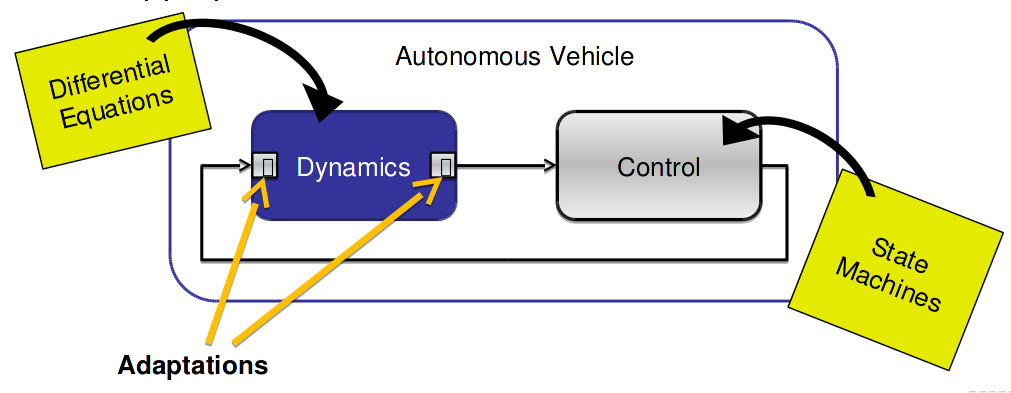
\includegraphics[scale=0.30]{images/intro}
\caption{Exemple d'adaptation sémantique dans un système.}
\label{fig:intro}
\end{figure}

\end{frame}


\section {Détails du sujet}

\begin{frame}
\frametitle{Détails du sujet (1)}

\begin{itemize}

  \item Simulation de systèmes mixtes: 

  \begin{itemize}
    
    	\item Problémes: modèles mathématiques différents. 
    	\item Côté analogique: algorithmes classiques de résolution d'équations
    	différentielles. Estimation de la valeur de la fonction pour chaque
    	instant de temps.  
    	\item Côté numérique: événements discrets. 
    	\item Exemple:
    	
    	\begin {center} 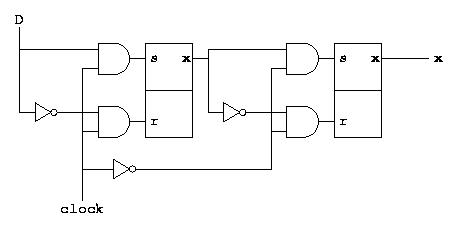
\includegraphics[scale=0.38]{images/analo} \end {center}
    	
    	\item 2 manières complètement effectuer les calculs: \\ (i) activer
    	le côté numérique après l'activation de l' analogique. \\  (ii)
    	n'activer la partie analogique que lorsqu'un événement discret est généré.
     
  \end{itemize}
  
\end{itemize}

\end{frame}

\begin{frame}
\frametitle{Détails du sujet (2)}

\begin{itemize}

  \item Théorie de \og l'Adaptation Sémantique \fg: réunir les concepts
  appartenant à un domaine spécifique et de les adapter à quelqu'un d'autre.
  \vspace{8pt}
  \item Adaptation en trois axes: temps, des données et de contrôle.
  \vspace{8pt}
  \item L'axe du temps: système responsable pour la conversion   d'un temps en
  secondes vers une rotation, càd, ce qu'on veut mesurer est le temps d'une
  rotation d'un engrenage par exemple.
  \vspace{8pt}
  \item L'axe des données: traduire une donnée analogique mesuré en volts à un
  niveau numérique binaire. Définir à partir de laquelle tension on
  considère le niveau binéaire comme 0 ou 1.
  \vspace{8pt} 
  \item L'axe du contrôle: façon dont les composants seront connectés dans le
  circuit et comment ils se communiquent. Par exemple : fil peut répresenter
  soit un bus de données ou soit une queue (\textit{FIFO}).


\end{itemize}
\end{frame}

\begin{frame}
\frametitle{Détails du sujet (3)}

\begin{itemize}

\item Les outils qui ont été développés:
\begin{itemize}
\vspace{5pt}
  \item \og MODELIX \fg~ : utilisé à \textit{Supélec}.
  \item \og PITOREMI \fg : développé à \textit{l'Université de Berkeley} aux
  États-Unis;
  \item \og SystemC \fg  \hspace{12pt}
  
\includegraphics[scale=0.3]{images/logo_systemc}
 
 \end{itemize}
\vspace{5pt}

\item Concepts relativement similaires, mais ils traitent le problème des façons
complètement différentes.

\vspace{5pt}

\item La solution développé est composée par:

\begin{itemize}
\vspace{5pt}
  \item Le schéma du circuit en haut niveau.
  \item La fonction sémantique de chaque composant (sa  signification dans le
  circuit).
 
 \end{itemize}
\end{itemize}
\end{frame}

\begin{frame}
\frametitle{Détails du sujet (4)}

\begin{figure}[h]
\centering
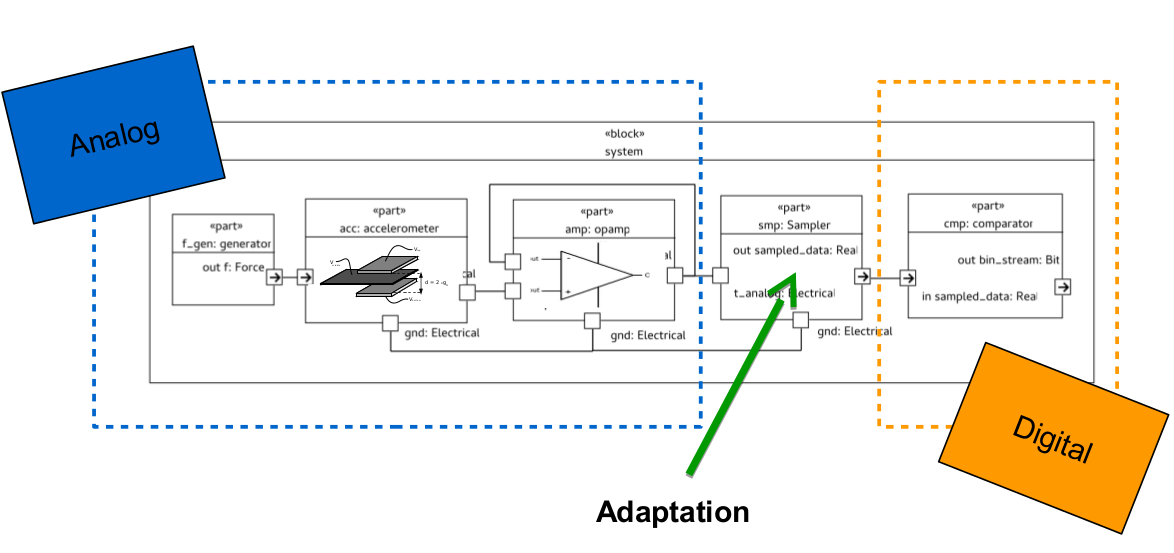
\includegraphics[scale=0.32]{images/exemple2}
\caption{Exemple modélisant l'adaptation entre systèmes continu et numérique.}
\label{fig:ex2}
\end{figure}

\end{frame}


\begin{frame}
\frametitle{Détails du sujet (5)}

\begin{itemize}
\item Capacité de spécification très puissante: on évite l'utilisation de
plusieurs simulateurs différents.
\item La simulation de systèmes très complexes, tels que des avions ou des
voitures devient plus simple et moins coûteuse. \\ \center{ \large{VALEUR
ÉCONOMIQUE}}
\end{itemize}

\begin{figure}[h]
\centering
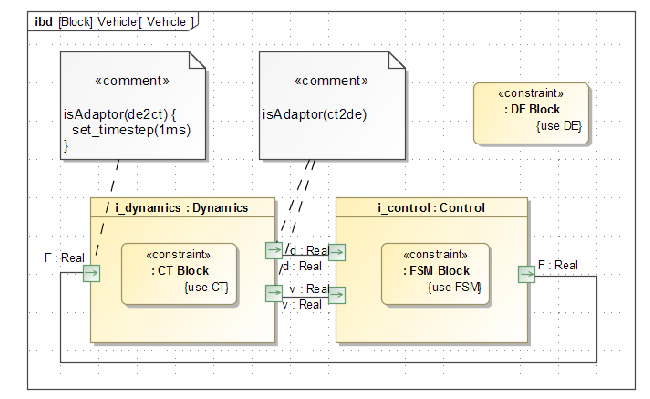
\includegraphics[scale=0.25]{images/exemple1}
\caption{Exemple modélisant l'adaptation entre deux systèmes d'une
voiture.}
\label{fig:ex1}
\end{figure}

\end{frame}


\section{Valorisation du sujet}

\begin{frame}
\frametitle{Valorisation du Sujet (1)}

\begin{itemize}

\item Document scientifique suit toujours un modèle: 
 
\begin{itemize}
  \item Introduction: expliquer brièvement le problème.
  \item Section dédiée à l'état actuel du problème: ce qui a été déjà
  développé et comment d'autres gens ont résolu ou sont en train de le faire. 
  \item Développement théorique et mathématique.
  \item Conclusion: perspectives futures. La partie la plus  importante d'un
  article vu qu'elle peut déterminer si l'article sera lu ou pas.

\end{itemize}

\item Plusieurs façons de publier un article - nous, en tant
qu'ingénieurs, avons deux objectifs principaux:

\begin{itemize} 
  \item l'IEEE \hspace{6cm}  
\includegraphics[scale=0.025]{images/IEEE_logo} \\
  		Séparer le texte en deux colonnes et bien énumérer la bibliographie. 
  \item l'ACM : (plutôt pour communauté informatique). \hspace{1pt}
  
\includegraphics[scale=0.2]{images/acm}\\
  		Écrire en une seule colonne avec la présence
de plusieurs espaces, ce qui permet l'utilisation des images par exemple

\end{itemize}

\end{itemize}

\end{frame}


\begin{frame}
\frametitle{Valorisation du Sujet (2)}

\begin{itemize}

\item  Revues ont différentes catégories et \og l'importance \fg~des articles publiés varient.

\begin{itemize}
  	\item \og\textit{Journals}~\fg~- les plus visés, ils sont publiés une fois
  	tous les 2 ou 3 ans. Ils ne contiennent que les meilleures recherches:
  	articles sont plus denses, + de 20 pages. 
	\vspace{8pt}
	\item Articles scientifiques de conférence: plus condensés et
	rapide (~ 8 pages). Suivi d'une présentation tenue par d'autres
	professionnels. 
	\vspace{8pt}
	\item L'article passe par un dernier examen final. Si tout est OK,
l'article est publié dans les \og~ \textit{transactions} ~\fg~ et tous ceux qui
sont inscrits dans la communauté peuvent y accéder. 
	\vspace{8pt}
	\item Le chercheur peut écrire des lettres courtes, en ajoutant de petits
	extraits à sa recherche (nouvelles idées, des suggestions, des résultats etc.).

\end{itemize}

\end{itemize}
\end{frame}

\begin{frame}
\frametitle{Valorisation du Sujet (3)}

\begin {itemize}
\item Le type de financement d'un doctorat: 

\begin {itemize} 
\item CIFRE:  collaboration entre l'établissement d'enseignement et la société.
Très ciblé, puisque les possibilités de développer sa carrière dans l'entreprise
sont hautes.

\item CNRS: financement consenti par le gouvernement et par l'école.

\vspace{12pt}
\begin{figure}[h]
\centering
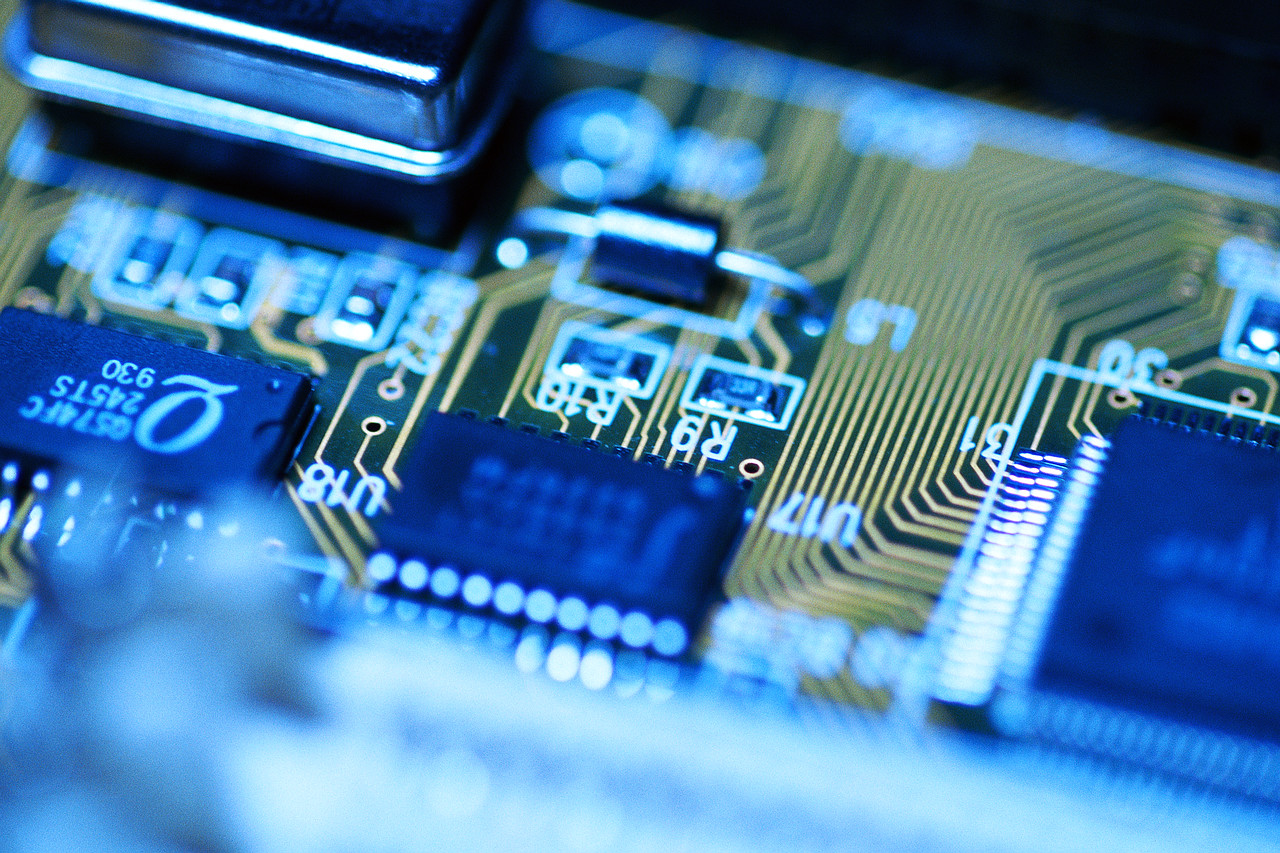
\includegraphics[scale=0.15]{images/lixo}
\end{figure}
\end{itemize}
\end{itemize}
\end{frame}

\section{Conclusions}

\begin{frame}
\frametitle{Conclusions}


\begin {itemize} 
\item L'activité de recherche assure la croissance et la réputation d'une
organisation grâce à son innovation.

\vspace{12pt}

\item L'aspect oral est aussi très important.

\vspace{12pt}

\item La recherche et l'industrie: complémentaires et, plus encore,
dépendent les unes des autres.

\end{itemize}
\end{frame}

\end{document}